\documentclass[11pt]{article}

\usepackage{hyperref}
\usepackage{graphicx}
\usepackage{color}
% \usepackage{fullpage}

\linespread{1.2}
\setlength{\parindent}{0pt}
\setlength{\parskip}{1.9ex plus 0.5ex minus 0.2ex}

% \newcounter{figure}
% \setcounter{figure}{1}

\begin{document}

\title{Compressing the Human Genome against a reference (draft-6)}
\author{Pragya Pande\\\texttt{\small{ppande@cs.stonybrook.edu}}\\\small{Stony Brook University} \and 
  Dhruv Matani\\\texttt{\small{dmatani@cs.stonybrook.edu}}\\\small{Stony Brook University}
}
\date{\today}

\maketitle

\vspace{0.5in}

\begin{abstract}
  We present a way to compress the complete human genome against a
  reference genome to achieve \textit{139x - 895x} compression. Our
  approach can potentially compress \textit{BUILD 36.3} of the human
  reference genome against (about \textit{2.6GiB}) \textit{BUILD 36.1}
  (also known as \textit{hg18}) to achieve a compression ratio of
  \textit{139x} (about \textit{19.2MiB}). The Korean genome
  \textit{KOREF\_20090224} (about \textit{2.9GiB}) can be compressed
  against \textit{KOREF\_20090131} to achieve a compression ratio of
  \textit{895x}, resulting in a file of size about
  \textit{3.3MiB}\footnote{These results are extrapolated from tests
    we ran on a subset of chromosomes for each genome pair}.

  The compressed differences are stored such that decompression from
  random offsets is fast. Furthermore, our \textit{range format} for
  storing differences allows us to \textit{efficiently} compute
  \textit{transitive differences} between the target genome and
  different reference genomes. Our method does not rely on the target
  genome being almost of the same size as the reference genome, or the
  existence of any alignment program available to us. We shall also
  prove that for the representation used, the technique we propose
  achieves optimal compression.

  We shall first motivate the problem itself, show existing research
  that has been done in this direction, present our approach, and
  compare it with prior work.

\end{abstract}

\setlength{\parskip}{0.7ex plus 0.5ex minus 0.2ex}

\clearpage

\tableofcontents

\setlength{\parskip}{1.9ex plus 0.5ex minus 0.2ex}

\clearpage

\section{Motivation}

The Complete Human Genome was sequenced in 2003. Since then a lot of
research is being done in genomics and computational biology. The
major input for most of the computation is the 2.9 billion base pairs
\cite{howmuchsequenced}\cite{findinghumangenome} of the human genome
which correspond to a maximum of about 725 megabytes of human
genome data.\cite{wikipediahumangenome}

Furthermore, reduction in the cost of sequencing (via the ``next-gen''
sequencing platforms) has given birth to the 1000 genomes project
\footnote{\url{http://www.1000genomes.org/}} which aims to sequence
the genomes of a large number of people. Just like the other human
genome reference projects, this data (estimated 8.2 billion bases per
day) would be made available via public databases for the scientific
community.\cite{1000genomes}

As we can now see, we are dealing with megabytes and megabytes of data 
when we work with genomes! This gives rise to challenging 
problems with respect to storage, distribution (downloading, copying), 
and sharing of this genomic data. Hence we need to consider better 
compression techniques for the genomic data. That apart, when working
with genomic data, we want to be able to optimize decompression so
that working with these compressed genomes is no harder than working
with the uncompressed genome.

The goal of the 1000 genomes project is to find most genetic variants
that have frequencies of at least 1\% in the populations
studied. Similarly, once the \$1000 genome
project\cite{1000dollargenomeproject} becomes successful, storage
costs for all the sequenced genomes will need to be kept under
control. To be able to do this, we need an space (and time) efficient
way of compressing the sequenced genomes so that the DNA of more
people can be sequenced for a reasonable price.

Multiple laboratories might use different reference genomes to
compress the genomes they sequence. For example, a Korean lab might
want to use a Korean genome as reference since it will be closer to
the genome of other Koreans. Other laboratories might have their own
reference genomes. However, if labs want to share sequenced genomes,
it becomes hard to share the difference compressed genome if the
differences have been computed with respect to different reference
genomes. One option is to decompress the sequenced genome and
re-compress it using the target reference as the reference
genome. However, since the compression is a time consuming process, we
would like to be able to quickly re-encode the genome with reference
to a difference reference genome.

We explore the problem of genome compression and see if we can:

\begin{itemize}

\item Better align 2 human genomes so as to facilitate better
  compression on them

\item Better compress the human genome to a smaller on-disk
  representation

\item Enable faster decompression

\item Enable space-efficient decompression

\item Enable I/O efficient decompression so that working with the
  compressed genome is the norm rather than the exception

\item Support \textit{efficient transitive compression} of a genome
  with respect to multiple reference genomes

\end{itemize}

\section{Existing Research}

\subsection{gzip \& bzip2}

These 2 applications are general loss-less compression routines that
use run-length encoding and block sort compression respectively. They
can compress the human genome (about 3GiB) to about 830MiB, which is a
compression ratio of \textit{3.67}.

\subsection{GenCompress, BioCompress \& Cfact}

GenCompress\cite{gencompress}, BioCompress\cite{biocompress} \&
Cfact\cite{cfact} are tools that mostly rely on either Huffman Coding,
Ziv-Lempel\cite{zivlempel}, or Arithmetic Coding to compress the human
genome. They are able achieve better compression when compared with
\textit{gzip \& bzip2}, but not as much as some of the difference
encoding methods mentioned below. These methods achieve compression
ratios of anywhere from \textit{4.82 -- 7.00}.

\subsection{Difference Encoding Techniques}

Difference encoding schemes are getting very popular since they can
achieve very high compression ratios of greater than \textit{100}
since \textit{99.9\%} of the genomes of 2 humans are similar to each
other. There are very few variations between the genomes of 2
individuals.

DNAzip\cite{dnazip}\cite{genomecompressionchenli} was the first
algorithm to compress the target genome by storing differences between
the target and reference genome. However, DNAzip does not solve the
problem of aligning 2 genomes with each other, but instead assumes the
existence of an \textit{SNP -- Single Nucleotide Polymorphism} file to
exist, which it takes in as input. In our experience, aligning 2
genomes is a very time consuming process and is orders of magnitude
slower than performing the actual compression itself.

Wang \& Zhang\cite{wangzhang} have come up with a difference
compression technique that is able to compress \textit{2986MiB} of a
Korean genome to \textit{18.8MiB}. This was done by difference
compressing the target genome it against another Korean genome which
was sequenced using similar methods and had the about the same
size. their technique considers blocks of bases of size 50, 20 or 10
million, and groups each chromosome from both the target and the
reference in these blocks to compute the difference between them. This
may not always work with genomes that have sequenced and assembled
using different techniques, or if you are using the human genome as a
reference to compress the mouse genome for example.

Researchers at Virginia Tech, Blacksburg\cite{vtechresearch} have
also come up with a difference compression algorithm that focuses on
decompression speed rather than raw compression ratio. We are also
motivated by some of the same factors that have motivated their
research. The technique presented achieves decompression times of
$O(\log{n})$ per random offset query. We also target a similar
complexity for random offset queries. They haven't publish exact
numbers on compressing the human genome, but claim that they achieve
\textit{98.8\%} compression when compressing mitochondrial sequences,
which roughly compresses the human genome of \textit{3GiB} to
\textit{36MiB}. Their technique also relies on align sequences of
chromosomes in the target with those in the reference genome. They use
the multiple sequence alignment application MUSCLE\cite{muscle} to
align the sequences with the reference genome.

Researchers at Cairo University, Egypt\cite{cairo} use existing
local-sequence-alignment programs to align the target and reference
sequence with each other. They then record insertions, deletions and
modifications with respect to the reference sequence and encode these
differences in a compact fashion. They have achieved \textit{99.4\%}
compression on the human genome, which means that they can compress
\textit{3GiB} of genomic sequence data to about
\textit{18.5MiB}. However, they don't talk much about decompression,
and it seems as if it is not entirely easy to decompress to random
offsets in the target genome. i.e. Ask for a sequence of length
\textit{l} at offset \textit{k} from the uncompressed genome.

\section{Our Solution}

\subsection{Outline of the Approach}

We compress the genome a chromosome at a time. $Ref_i$ is our
reference chromosome and $Victim_i$ is the chromosome to be
compressed.

We shall find the optimal (least) number of ranges from $Ref_i$ that
can completely cover $Victim_i$. To do this, we shall construct a
Suffix Array on $Ref_i$ \& $Victim_i$ and then find the least range
covering. We shall prove that for an encoding that only encodes
\textit{(offset, length)} pairs from the reference, this
representation is optimal in terms of the number of ranges needed to
completely cover the entire target chromosome.

Subsequently, the plain-text file containing these optimal number of
ranges is encoded in a binary format and the resulting binary file is
further compressed using \textit{gzip} to produce the final compressed
difference file.

Hence, it is easy to see that our approach will provide good
compression as long as there is a sufficient amount of overlap between
the target and reference genomes even if:
\begin{itemize}
\item The 2 genomes have different lengths.
\item The genomes have been sequenced and assembled using different
  apparatus and methods.
\item You try to compress the mouse genome with a human genome as a
  reference.
\end{itemize}

\begin{figure}
  \begin{center}
    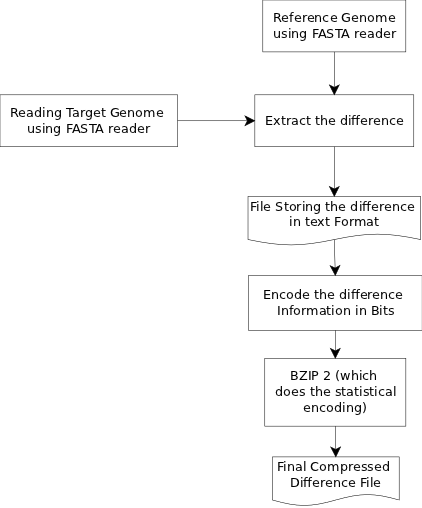
\includegraphics[height=4.1in]{figures/GenomeCompressionFlow.png}
    \caption{The flow of Genome Compression}
    \label{fig:genomecompressionflow}
  \end{center}
\end {figure}

\clearpage

\subsection{The Algorithm}

\begin{enumerate}

\item For each corresponding chromosome pair ${Ref}_i$ \& $Victim_i i
  \in [1\ldots{}23]$, build a
  \textit{suffix array}\footnote{This is done using Manber \& Myers
    $O(n\log{n})$ suffix array construction
    algorithm\cite{manbermyers}, which allows us to compute the
    \textit{Longest common Prefix} of 2 adjacent suffixes in
    $O(\log{n})$ time} from the string $Ref_i\#Victim_i\$$.

\item For every suffix in ${Victim}_i$, find the length of the longest
  prefix that matches with some string at index $j$ in ${Ref}_i$.

\item Now that we have all the ranges in $Ref_i$ that $Victim_i$ can
  be covered by, we find the least number of ranges that can
  completely cover $Victim_i$. This can be done in
  $O(n\log{n})$\footnote{There is also a (single-pass) $O(n)$
    time algorithm to do the same, but we don't talk about it here}
  time using \textit{Dynamic Programming} and \textit{Segment Trees}
  as an online \textit{Range Minimum Query} data structure. The
  problem of finding the minimal number of completely covering
  sub-ranges exhibits optimal substructure. i.e. A solution for the
  range $[i\ldots{}n]$ can be constructed using the solution to the
  ranges $[i+1\ldots{}n], [i+2\ldots{}n], [i+3\ldots{}n], \ldots{},
  [i+k-1\ldots{}n]$, where $k$ is the length of the range starting at
  index $i$.

\end{enumerate}

\subsection{Transitive Difference Computation}

Suppose \textit{V} is the victim genome that is already compressed
with reference to the reference genome \textit{$R_1$}, and we want to
compress it with respect to reference genome \textit{$R_2$}, then we
need to compute how genome \textit{$R_1$} compress with respect to
genome \textit{$R_2$}. Since we expect to compress many victims with
respect to a fixed number of variable references, we can ignore the
cost of computing this difference. Besides, this is just a one time
process and once the delta \textit{$R_1 - R_2$} has been computed, we
can reuse it indefinitely.

\begin{figure}
  \begin{center}
    \includegraphics[height=2.5in]{figures/TransitiveDifference.png}
    \caption{Transitive Difference Computation}
    \label{fig:transitivedifferencecomputation}
  \end{center}
\end {figure}

To be able to compute transitive differences, we need to slightly
modify the output of the compression routine. Instead of storing just
the tuple \textit{(offset, length)}, we store the tuple
\textit{(offset, length, span)}, where \textit{span} is the actual
span of the range (length of maximum match) between the victim and
reference. This span is the value computed using the suffix array and
longest common prefix algorithm.

Now, given the files \textit{$V - R_1$} and \textit{$R_1 - R_2$}, we
need to find, for every offset \textit{i} in \textit{V}, in index
\textit{j} in \textit{$R_1$} where it can be found. Once we know the
value of \textit{j}, we lookup \textit{$R_1 - R_2$} to locate the
index \textit{k} in \textit{$R_2$} of the index \textit{j} in
\textit{$R_1$}. This lookup need not be done on a per index basis, but
can instead be done on a range basis. This is an optimization that
reduces the running time of this algorithm.

Each lookup into the difference file \textit{$R_1 - R_2$} costs
$O(\log{n})$, (where $n$ is the number of lines in \textit{$R_1 -
  R_2$}) and we need to process \textit{$O(m)$} such ranges (since
ranges may get split during this operation). Here, $m$ is the total
number of lines in the file \textit{$V - R_1$}. Hence, the total
running time of the transitive difference computation routine is
$O(m\log{n})$.

We must mention however that the differences computed using the
transitive difference routine are \textit{not} optimal.

\subsection{Proof of Optimality}

We shall prove by contradiction that for the range based encoding
scheme we have used, the algorithm presented above achieves optimal
compression in terms of the number of ranges used to represent the
completely covered \textit{victim} chromosome.

Given the following range lengths starting at the indexes at which
they occur, what is the least number of ranges that completely cover
the whole range?

\begin{center}
  \begin{tabular}{|l|c|c|c|c|c|c|c|c|c|c|c|c|c|c|c|}
    \hline
    Index        & 0 & 1 & 2 & 3 & 4 & 5 & 6 & 7 & 8 & 9 &10 &11 &12 &13\\
    \hline
    Range Length & 3 & 2 & 4 & 1 & 1 & 1 & 3 & 6 & 8 & 2 & 1 & 2 & 1 & 1\\
    \hline
  \end{tabular}\\
  \vspace{0.3cm}

  \addtocounter{figure}{1}
  \footnotesize{Figure-\arabic{figure}: Indexes and lengths of ranges
    at those indexes}
\end{center}

The best solution extends the smallest range that it can cover to its
right.

\begin{center}
  \begin{tabular}{|l|c|c|c|c|c|c|c|c|c|c|c|c|c|c|c|}
    \hline
    Index         & 0 & 1 & 2 & 3 & 4 & 5 & 6 & 7 & 8 & 9 &10 &11 &12 &13\\
    \hline
    Range Length  & 3 & 2 & 4 & 1 & 1 & 1 & 3 & 6 & 8 & 2 & 1 & 2 & 1 & 1\\
    \hline
    Min n(Ranges) &  &  &  &  &  &  &  & \textcolor{red}{2} & \textbf{\textcolor{red}{1}} & \textcolor{red}{3} & 3 & 2 & 2 & 1\\
    \hline
  \end{tabular}\\
  \vspace{0.3cm}

  \addtocounter{figure}{1}
  \footnotesize{Figure-\arabic{figure}: If we have the solution till
    index $7$, and we want to extend it to compute the solution till
    index $6$, then we scan up to $3$ (the length of the longest range
    at index $6$) places to the right of index $6$ (shown in
    \textcolor{red}{red}), and locate the smallest value in that range
    (shown in bold face).}
\end{center}


\begin{center}
  \begin{tabular}{|l|c|c|c|c|c|c|c|c|c|c|c|c|c|c|c|}
    \hline
    Index         & 0 & 1 & 2 & 3 & 4 & 5 & 6 & 7 & 8 & 9 &10 &11 &12 &13\\
    \hline
    Range Length  & 3 & 2 & 4 & 1 & 1 & 1 & 3 & 6 & 8 & 2 & 1 & 2 & 1 & 1\\
    \hline
    Min n(Ranges) & 4 & 4 & 3 & 5 & 4 & 3 & 2 & 2 & 1 & 3 & 3 & 2 & 2 & 1\\
    \hline
    Next Index    & \textcolor{red}{3} & 2 & \textcolor{red}{6} & 4 & 5 & 6 & \textcolor{red}{8} & 8 & \textcolor{red}{14} &10 &11 &13 &13 &14\\
    \hline
  \end{tabular}\\
  \vspace{0.3cm}

  \addtocounter{figure}{1}

  \footnotesize{Figure-\arabic{figure}: The numbers in
    \textcolor{red}{red} indicate the range end-points that make up
    the ranges that cover the entire sequence. If \textit{n} numbers
    make up the range, then there exist \textit{(n-1)} ranges. Range
    extension stops when we have gone past the last index in the
    sequence (14 in this example).}

\end{center}

If there is a better solution at any stage, then it would have been
the one chosen by our algorithm for extending a range from a given
index.

\subsection{Binary Encoding}

We use a tight binary format to represent the \textit{(offset,
  length)} pairs into the reference that are needed to represent the
target genome.

Each line in the intermediate plain-text range file holds an
\textit{(offset, length)} pair that needs to be encoded. Since offsets
can be quite large, we always encode them as fixed 32-bit
integers. The length values however have a different distribution. For
a chromosome we compressed, here is the distribution of length values.

\begin{center}
  \begin{tabular}{|c|c|c|c|}
    \hline
    Range of Values & [1\ldots{}127] & [128\ldots{}16383] & [16384\ldots{}]\\
    \hline
    Counts & 56620502 & 60686338 & 2602\\
    \hline
    Percentages & 48.27\% & 51.73\% & 0.0022\%\\
    \hline
  \end{tabular}\\
  \vspace{0.3cm}

  \addtocounter{figure}{1}
  \footnotesize{Figure-\arabic{figure}: Distribution of length values
    in the compressed ranges file.}

\end{center}

All values in the range [1\ldots{}127] are encoded as a single byte
integer with the MSB set to \texttt{1}. Values in the range
[128\ldots{}16383] are encoded as 2-byte integers, with the first 2
most significant bits set to \texttt{01}. Values greater than 16383
are encoded as 4-byte integers with the first 2 most significant bits
set to \texttt{00}. This allows us to uniquely identify the size of
the value based just on the value of the 2 most significant bits of
the integer.

\subsection{Decompression}

The difference encoded file looks like this:
\begin{verbatim}
61771 51
7829  89
17288 12
7288  6523
\end{verbatim}

These are ranges with lengths 51, 89, 12, \& 6523. We construct an
intermediate file containing the cumulative lengths to allow quick
random retrieval. The pre-processed data looks like this:

\begin{verbatim}
61771 0
7829  51
17288 140
7288  152
--    6675
\end{verbatim}

Now, to get the decompressed chromosome data of length 100 at offset
130, we need to just do a \textit{Binary Search} into the cumulative
length array and find the location of offset 130. This happens to be
at offset 7829+79 in the reference file. The range of length 200
happens to span 3 ranges, one is the previous range, and the other
ones are at offset 17288 with length 12 and offset 7288 with length
109. Since all the blocks in the reference come from the same
chromosome, we can prevent disk seeks by loading the whole chromosome
into memory before starting decompression (or alternatively incur a
cost of a few disk seeks per retrieval). If we consider the case where
we have many genomes compressed with respect to a fixed reference
genome, then it is sufficient to just keep that genome, and all the
difference files in memory to ensure fast random \& sequential
decompression.


\subsection{Practical Considerations}

Every chromosome of the target genome was stripped off any \textit{N}
characters (unknown base-pair) before compressing it against the
reference genome's corresponding chromosome. These unknown base-pairs
mostly occur at the beginning and end of each chromosome.

We ran the experiments on a 32-bit VMWare Player Virtual Machine
running Ubuntu 11.04, with Windows 7 as the Host Operating
System. Since the guest is a 32-bit system, the process address space
is limited to 4GiB, out of which about 1.5GiB of the higher address
space is used up by the kernel and dynamically loaded libraries such
as \textit{glibc}, etc\ldots{}. This leaves us with 2.5GiB to
use. When constructing the Suffix Array, we have observed that there
are rarely sub-strings greater than \textit{65,536} in length that
overlap in 2 genomes. This means that we can cap the extra space
required by the suffix array construction algorithm to $16n \times
sizeof(int)$. An additional $3n$ space overhead is incurred to store
the input string and a $5n \times sizeof(int)$ overhead is incurred
while computing the optimal overlap of ranges.

All this adds up to (in bytes):\\
$16n \times sizeof(int) + 3n + 5n \times sizeof(int)$\\
$= 16n \times 4 + 3n + 5n \times 4$\\
$= 64n + 3n + 20n$\\
$= 87n$\\

Hence, the space requirement for our algorithm is $O(n)$, with a
fairly high constant overhead.

Equating the 2 sides, we get:\\
$2.5 \times 1024^3 = 87n$\\
Solving for $n$, we get:\\
$n = 30854650$\\
which translates to about \textit{30 million}.

Hence, we can process only strings of length \textit{30 million} at a
time with the process address space that we have.

Experimentally, we determined that we got the best results if we chose
\textit{16MiB} of data from the reference chromosome \& \textit{6MiB}
of data from the target chromosome (totaling \textit{22MiB} in
all). We had to rune some more experiments to find out the best way to
align these blocks so that maximum compression for the target could be
achieved. We found that we occasionally need to align each block of
\textit{6MiB} with potentially \textit{2--3} blocks of size
\textit{16MiB} from the reference to get the best
compression. Generally \textit{uncompressed plain-text} difference
files for \textit{6MiB} from the target range anywhere from
{\textit{90KiB to 300KiB}}. If we see results in this range, we don't
try other ranges.

This \textit{block based} processing of the chromosomes results in
sub-optimal compression, but:
\begin{itemize}
\item Allows us to work around process address space limits even
  though the machine might have enough physical memory.
\item Results in faster decompression since the hard disk needle need
  not seek too far (the 16MiB block from which the differences are
  generated is all that is needed to decompress a 6MiB block). This
  makes decompression a very \textit{I/O-efficient} process.
\end{itemize}

Compressing a \textit{full} target chromosome against another
\textit{full} reference chromosome will result in better compression,
but will require more memory during decompression (or will result in
more disk seeks if available memory during decompression is bounded).

You can see that by varying these block sizes, one can achieve a
balance between compression ratio and decompression speed/memory
required to compress \& decompress a chromosome.


\section{Approaches Compared}

\subsection{DNAzip}

The DNAzip group relies on an existing \textit{SNP} file being
present, and hence they don't do sequence alignment before compressing
the difference file.

It isn't possible to trivially get the decompressed genome data at a
certain \textit{(offset, length)} pair without decompressing the
complete genome.

\subsection{Wang \& Zhang's method}

Wang \& Zhang's method is called \textit{The GRS tool} and it works in
blocks of size 50, 25, or 10 million. It relies on being able to
compute the longest common sequence between 2 blocks. It isn't
immediately apparent how easy it would be to support fast \& efficient
random offset querying on the compressed data generated by \textit{The
  GRS tool}.

\subsection{Virginia Tech Research}

The approach that the Researchers at Virginia Tech,
Blacksburg\cite{vtechresearch} use is one of using existing sequence
alignment programs such as MUSCLE\cite{muscle} to do the heavy lifting
of aligning sequences with each other and then encode the differences
using one of the following 5 operators:
\begin{enumerate}
\item insertion
\item deletion
\item replacement
\item insertion after replacement, and
\item deletion after replacement
\end{enumerate}

These difference operations are then tightly compressed using
\textit{Huffman Compression} to produce the final output.

The highlight of their approach is that they support very fast random
offset decompression.

\subsection{Tabulated Comparison}

\begin{center}
  \begin{tabular}{|p{0.6in}|p{0.7in}|p{0.5in}|p{0.8in}|p{0.5in}|p{0.9in}|p{0.9in}|}
    \hline
    Method & Does Sequence Alignment & Works on FASTA & Human Genome
    Compressed to & Comp. Ratio & Fast Decompression & Random
    Offset Querying\\
    \hline
    DNAzip & No & No & 4.1MiB & 724 & Yes & No\\
    \hline
    GRS & Yes & Yes & 18.8MiB & 159 & Yes & Not clear\\
    \hline
    VTech & Yes & Yes & 36MiB & 85 & Yes & Yes $O(\log{n})$\\
    \hline
    Cairo & Yes & Yes & 18.5MiB & 166 & Yes & No\\
    \hline
    Proposed & Yes & Yes & 22MiB & 139 & Yes & Yes $O(\log{n})$\\
    \hline
  \end{tabular}\\
  \vspace{0.3cm}

  \addtocounter{figure}{1}
  \footnotesize{Figure-\arabic{figure}: A comparison of various
    approaches}

\end{center}


\section{Experimental Results}

When run on \textit{hg18} as the reference genome and \textit{BUILD
  36.3} of the human genome reference as the target genome, here are
the results we got for some chromosomes.

\begin{center}
  \begin{tabular}{|c|r|r|r|}
    \hline
    Chromosome & Original (MiB) & Compressed (KiB) & Compression
    Ratio\\
    \hline
    14 & 83 & 554 & 153.4\\
    \hline
    15 & 73 & 562 & 133.0\\
    \hline
    20 & 57 & 387 & 150.8\\
    \hline
    21 & 32 & 219 & 149.6\\
    \hline
    22 & 32 & 243 & 134.8\\
    \hline
  \end{tabular}\\
  \vspace{0.3cm}

  \addtocounter{figure}{1}
  \footnotesize{Figure-\arabic{figure}: Compression of certain human
    chromosomes.}

\end{center}


When run on \textit{KOREF\_20090131} as the reference genome and
\textit{KOREF\_20090224} as the target genome, here are the results we
got for some chromosomes.

\begin{center}
  \begin{tabular}{|c|p{0.75in}|p{0.9in}|p{1in}|p{1in}|}
    \hline
    Chromosome & Compressed (KiB) & Compression
    Ratio & GRS Compressed (KiB) & GRS Compression Ratio\\
    \hline
    16 & 97 & 918.43 & 554.7 & 158.9\\
    \hline
    17 & 86 & 893.02 & 494.1 & 158.3\\
    \hline
    18 & 73 & 1009.97 & 399.0 & 189.4\\
    \hline
    22 & 48 & 682.67 & 256.3 & 192.6\\
    \hline
  \end{tabular}\\
  \vspace{0.3cm}

  \addtocounter{figure}{1}
  \footnotesize{Figure-\arabic{figure}: Comparison of compression
    achieved by our method v/s that achieved by the \textit{GRS Tool}
    on certain chromosomes sequenced from Korean
    individuals. Chromosome 16 was NOT stripped off the \textit{N}
    characters to show that removing these characters doesn't the
    compression ratio.}

\end{center}


\section{Future Work}

Compressing the genome \textit{6MiB} at a time against \textit{16MiB} of
data from the reference takes about \textit{15.5 minutes} on a single
core (CPU).

This computation can be parallelized across multiple cores. If the
compression is being done a chromosome-at-a-time, then each chromosome
can be processed on a separate CPU so that the total time required is
the \textit{maximum} of the time required to compress each chromosome
rather than the \textit{sum} of their times.

\section{Acknowledgments}

We would like to thank Dr. Skiena for giving us the opportunity to
work on this project and rightly penalizing us for a less-than-optimal
project proposal \& progress report. This made us work harder on the
project. Though, we would like to believe that the real reason for our
earlier lethargy was the phenomenon of \textit{Temporal
  Discounting}\footnote{\url{http://en.wikipedia.org/wiki/Temporal_discounting}:
  Temporal discounting refers to the tendency of people to discount
  rewards as they approach a temporal horizon in the future or the
  past (i.e., become so distant in time that they cease to be valuable
  or to have additive effects).}

We would also like to thank Aniruddha Laud, Gaurav Menghani, \&
Madhava K R, who patiently explained the working of
DNAzip\cite{dnazip} to us.



\clearpage

\begin{thebibliography}{9}

\bibitem{dnazip} DNAzip: DNA sequence compression using a reference
  genome \url{http://www.ics.uci.edu/~dnazip/}
\bibitem{howmuchsequenced}
How much of the human genome has been sequenced?
\url{http://www.strategicgenomics.com/Genome/index.htm}
\bibitem{findinghumangenome}
Finishing the euchromatic sequence of the human genome
\url{http://www.nature.com/nature/journal/v431/n7011/abs/nature03001.html}
\bibitem{wikipediahumangenome}
Wikipedia on The Human Genome
\url{http://en.wikipedia.org/wiki/Human\_genome}
\bibitem{1000genomes}
The 100 genomes project aims to provide a comprehensive resource on
human genetic variation. \url{http://www.1000genomes.org/about}
\bibitem{zivlempel}
A Universal Algorithm for Sequential Data Compression, IEEE
Trans. Information Theory, vol. 23, pp. 337-343, 1977.
\bibitem{gencompress}
DNABIT Compress -- Genome compression algorithm. Pothuraju
Rajarajeswari and Allam Apparao
\bibitem{biocompress}
A New Challenge for Compression Algorithms: Genetic Sequences,
S. Grumbach and F. Tahi, Information Processing Management, vol. 30,
no. 6, pp. 875-886, 1994.
\bibitem{cfact}
A Guarantee DNA Sequences for Repetitive DNA Sequences, E. Rivals,
J.P.Delahaye, M.Dauchet, and O.Delgrange, LIFL Lille I University,
Technical Report IT-285, 1995.
\bibitem{1000dollargenomeproject}
Anticipating the 1,000 dollar genome, Mardis ER
\bibitem{wangzhang}
A novel compression tool for efficient storage of genome resequencing
data. Congmao Wang and Dabing Zhang
\bibitem{vtechresearch}
A Genome Compression Algorithm Supporting Manipulation. Lenwood
S. Heath, Ao-ping Hou, Huadong Xia, and Liqing Zhang
\bibitem{muscle}
MUSCLE: Multiple sequence alignment with high accuracy and high
throughput, R. C. Edgar, Nucleic Acids Research, 32 (2004),
pp. 1792–1797.
\bibitem{cairo}
DNA Lossless Difference Compression Algorithm Based On Similarity Of
Genomic Sequence Database, Heba Afify, Muhammad Islam, and Manal Abdel
Wahed
\bibitem{manbermyers}
Suffix arrays: A new method for on-line string searches, Udi Manber
and Gene Myers
\bibitem{genomecompressionchenli}
Human genomes as email attachments.
Scott Christley, Yiming Lu, Chen Li, \and Xiaohui Xie


\end{thebibliography}

\end{document}
